\documentclass{article}
\usepackage{hyperref}
\usepackage{graphicx}
\usepackage{geometry}

 \geometry{
 a4paper,
 left=20mm,
 right=20mm,
 top=20mm,
 }
 
\hypersetup{
    colorlinks,
    citecolor=black,
    filecolor=black,
    linkcolor=black,
    urlcolor=black
}

\begin{document}

    \section{Subsystems}
    
    \subsection{Events Subsystem}
    
    \subsubsection{Overview}
    
    The events module serves as the system to log, update and view events that might be hosted on the University. These events include Educational and Social events, but can be branched out to other categories as they arise.
    
    \subsubsection{UML Diagrams}
    
    \begin{figure}[h!]
        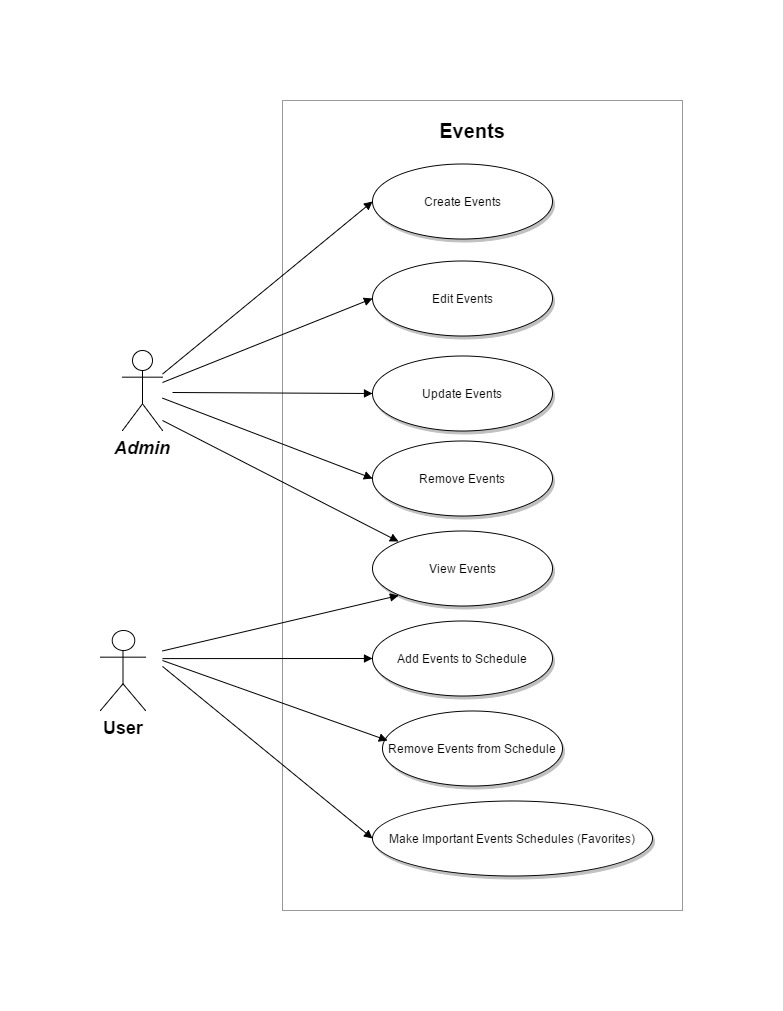
\includegraphics[width=0.8\textwidth]{Images/EventUC.jpg}
    \end{figure}
    Events Use Case Diagram
    
    \mbox{}\\
    \bigskip
    \clearpage
    
    \begin{figure}[h!]
      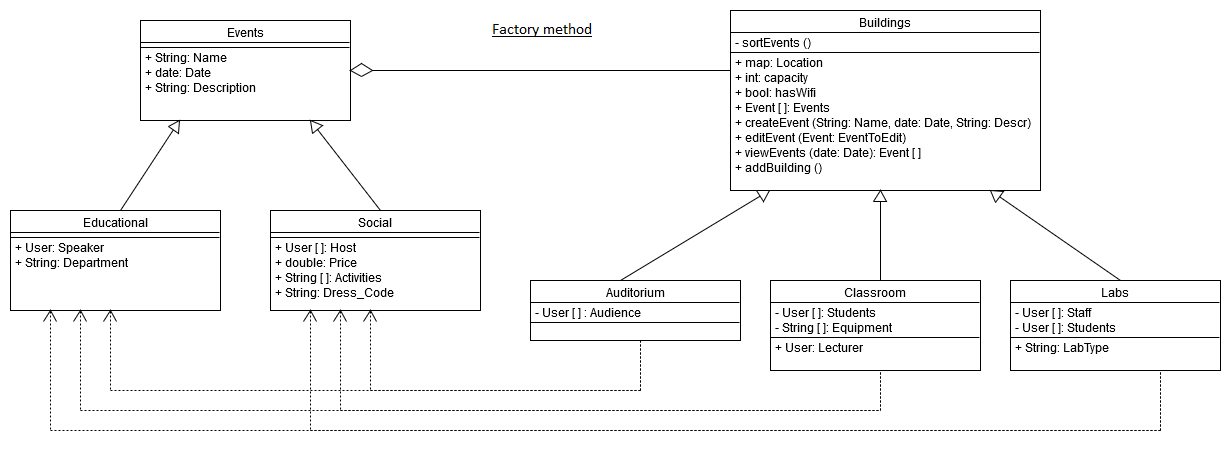
\includegraphics[width=\textwidth]{Images/ClassDiagramEvents.png}
    \end{figure}
    Events Class Diagram
    
    \begin{flushleft}
    
        For the events subsystem the Factory Method design pattern is applicable, as this pattern allows objects of the same abstract type to be initiated by letting a certain framework or object user decide which type of concrete class to instantiate.
        
        \bigskip
        
        In this instance, a certain type of building is allowed to host an event of a certain type. This allows for greater accuracy in searching for a certain event in a certain building. It also enables the events to be easily sorted and ordered to make presentation to the user easier. The fact that buildings as well as events can be created or altered dynamically also is catered for by the Factory Method, since a concrete building can easily be created and linked to the relevant concrete event, which can also be created and destroyed with ease. This is done while still maintaining the relevant needed information and functionality that each building and event needs (which is hosted in the abstract class).
        
        \bigskip
        
        There are methods in the Buildings class that allow users to add buildings as they are needed. The Buildings class also allows users to edit, view or add Events. This is done in the Building class as it is implemented with the Framework role of the design pattern. The viewEvents() function will act as a searcher function that will traverse the list of events that the relevant building is hosting in order to enable a user to invoke other functionalities, like  viewing an event or editing an event. The Buildings class can be called from any other module that would like to have access a to Events, like if the User class wants to add an event.
        
        \bigskip
        Notify: Subject
        
        Send Notification: Observer(Observer) / Abstract Method(Template)
        
        Send Email: Concrete Observer1(Observer) /Concrete Method(Template)
        
        Send SMS: Concrete Observer2(Observer) / Concrete Method(Template)
    
    \end{flushleft}
    
    \mbox{}\\
    \bigskip
    \clearpage
    
    \begin{figure}[h!]
        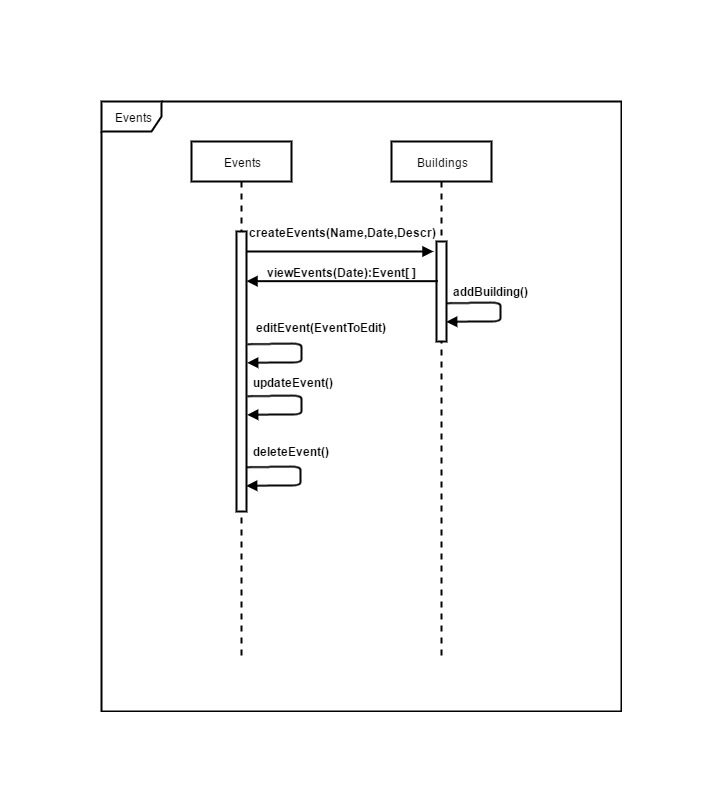
\includegraphics[width=\textwidth]{Images/EventsSequence.jpg}
    \end{figure}
    Events Sequence Diagram
    
    \mbox{}\\
    \bigskip
    \clearpage
    
    \begin{figure}[h!]
        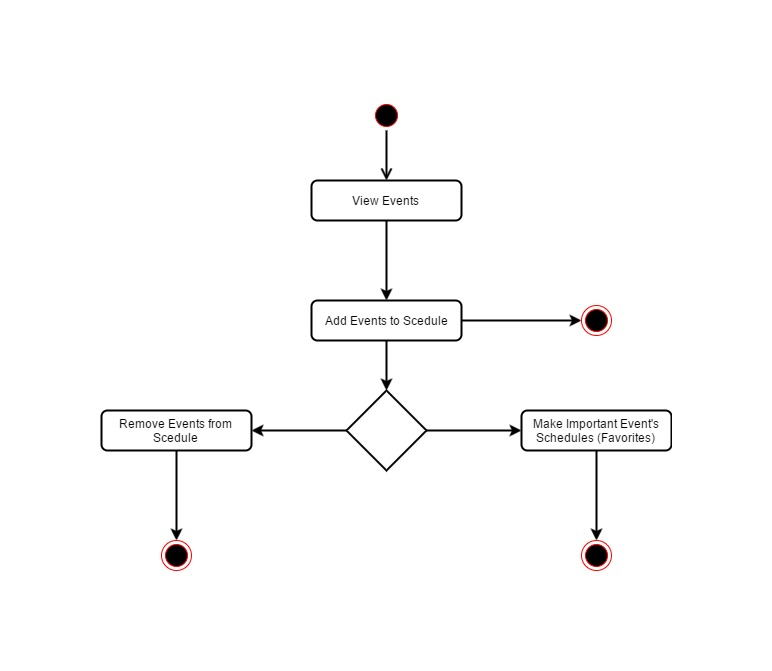
\includegraphics[width=\textwidth]{Images/ActivityDiagramUser.jpg}
    \end{figure}
    Normal User Activity Diagram
    
    \mbox{}\\
    \bigskip
    \clearpage
    
    \begin{figure}[h!]
        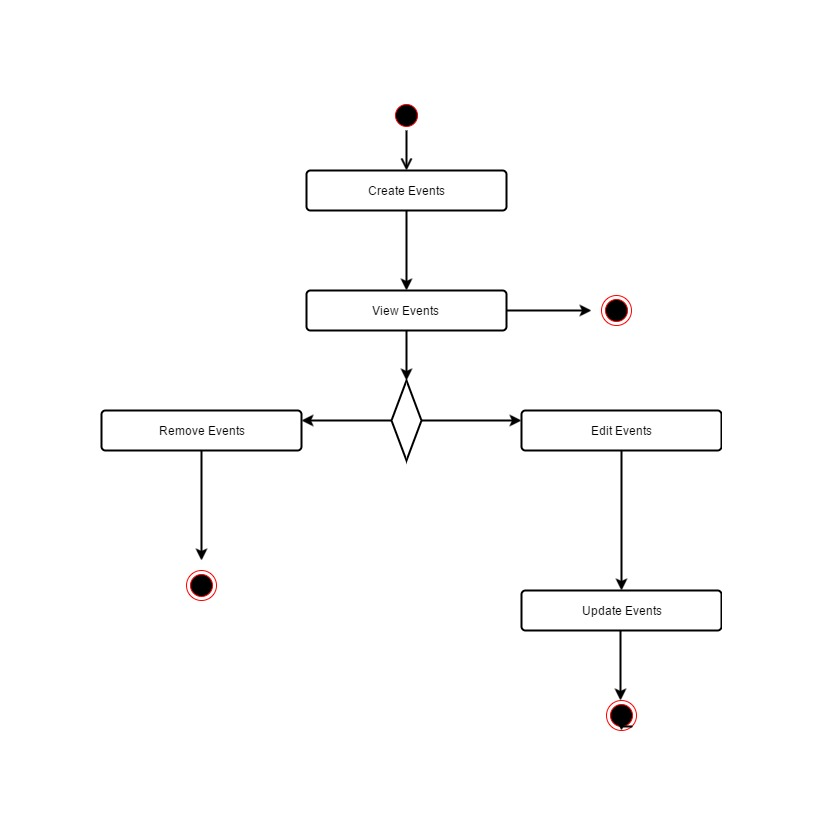
\includegraphics[width=\textwidth]{Images/ActivityDiagramAdmin.jpg}
    \end{figure}
    Advanced User Activity Diagram
    
    \mbox{}\\
    \bigskip
    \clearpage
    
    \begin{figure}[h!]
        \begin{center}
            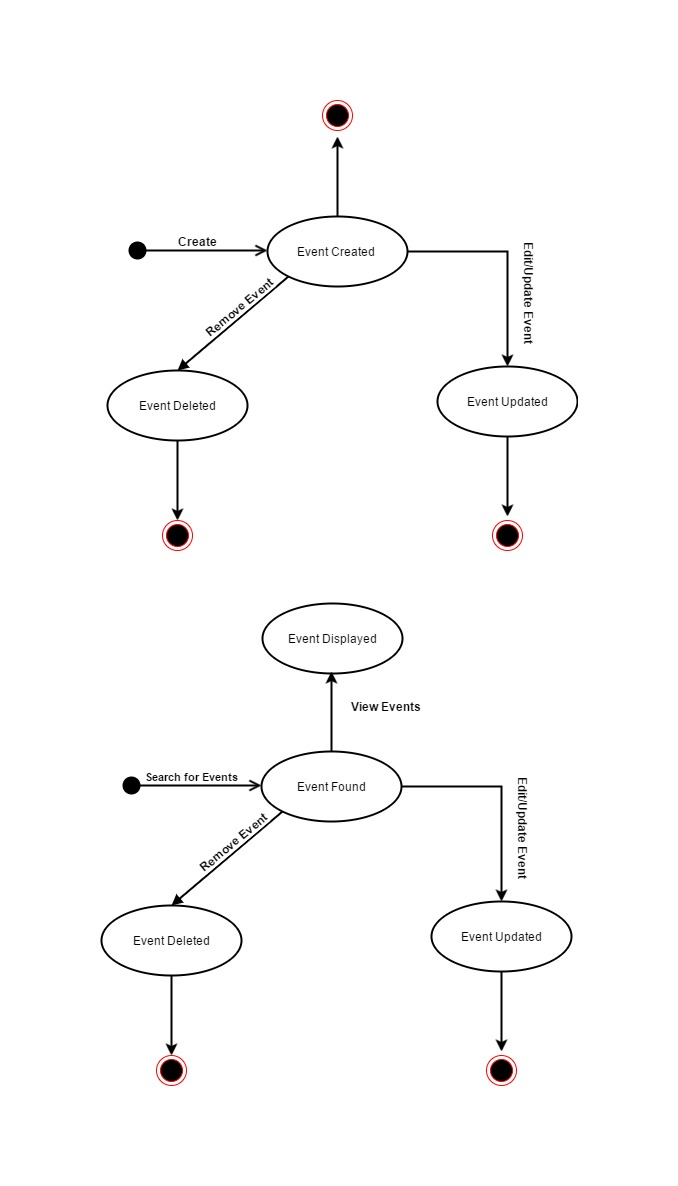
\includegraphics[width=0.6\textwidth]{Images/StateDiagramEvent.jpg}
        \end{center}
    \end{figure}
    Events State Diagram
    
    \mbox{}\\
\end{document}
